\section{The GPU-Centric Design}
\subsection{Design Principle}
The design of AVIST follows two important principles: 1) \textit{fully utilizing the GPU  fine parallelism and high memory bandwidth to boost performance on a commodity desktop computer}; 2) \textit{affording flexible visual querying and filtering, such as animation and cross-filtering, to visually explore fine level data details}. Based on these two guidelines, we carefully consider the data storage and computation design on the GPU:
\begin{itemize}
\item  \textbf{Data storage}:  We store  raw data on the GPU memory. Moreover, all derived data are also on the GPU memory to fully take advantage of the GPU high memory bandwidth.


\item \textbf{Data computation}: We highlight cross-filtering  for slicing data records from different attributes (animation for time domain). A data dependency graph (directed acyclic graph) characterizes such data transformations on the GPU to support data aggregation and visualization on demand.

\end{itemize}

\subsection{The GPU-Centric Design}

There are two key ideas about the GPU-centric design: 1)  raw data is stored on the GPU memory; and 2) data processing is parallelized on the GPU.

We emphasize that the raw data is important for exploratory visual analysis. Because it can potentially help analysts to analyze each data record without any information loss (\textit{finding a needle in haystack}).  The raw data is stored in the GPU memory, which enables: 1) fast data accessing based on its high bandwidth; and 2) avoiding data transfers between CPU and GPU. Besides the raw data,  the derived data is also stored on the GPU memory (visual primitives are stored on the GPU vertex buffer objects). 

We also highlight that data aggregation and visualization are  based on the GPU parallel computing. The benefits include: 1) vectored computing for utilizing the GPU fine level parallelism; 2) data aggregations  and visualizations are on demand rather than precomputation.


\begin{figure}[htb]
	\centering
	
	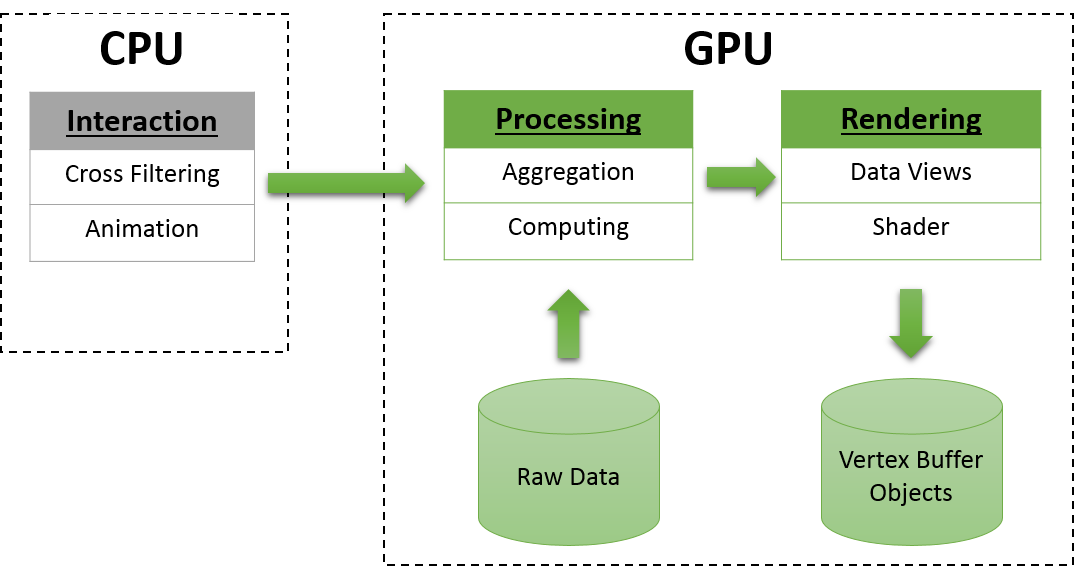
\includegraphics[width=1.0\linewidth]{pic/arch.png}
	\parbox[t]{1.0\columnwidth}{\relax
	}
	%
	\caption{\label{fig:architecture} The GPU-centric design: user interactions are transfered from the CPU to the GPU. Data storage and computation are on the GPU. }
\end{figure}


Figure~\ref{fig:architecture} shows the GPU-centric design. User interactions are generated in the CPU side, then they are transfered into the GPU, which triggers the GPU parallel processing and rendering.
The GPU is the main platform for data storage and  computing. 
The data resides on the GPU memory for fast fetching, which are mainly about raw data and visual primitives.  The GPU computation is also separated into two parts: 1) the general data aggregation and filtering; 2) the computation of each data view for generating visual primitives.  
%The GPU parallel computing is on the fly,  which is caused by user interactions (animation and cross filtering).  
In all, the GPU-centric design emphasizes that both data storage and processing are handled by the GPU, which fully utilizes the GPU  parallelism and high memory bandwidth.

\subsection{Data Storage}
As we mentioned, the GPU memory capacity limits the GPU-centric design for handling even larger datasets.  To feed more data into the GPU memory, we apply a lossless compression technique for preprocessing  multidimensional datasets. 

  

Consider a multi-dimensional dataset, which may include different types of data.  Firstly, we identify each data type, which can be separated into time data, quantitative data, and categorical-ordinal data. Secondly, we use different methods for compressing those types of data based on their characteristics.    
Considering the categorical-ordinal data, we count  all possible values and map each value into a unique ID. This  key-value map is stored in main memory as meta data.  We calculate the minimum and maximum values for time and quantitative data, and store them in main memory as  meta data.    
 
On the GPU side, we organize the raw data in a row-oriented format, where all data records are ordered by their time values (we emphasize the data temporal and spatial locality for fast data retrieving and processing). We store each data item's binary code instead of its ASCII code for saving memory space. Thus, each time data item occupies 8 bytes; each quantitative data needs 4 bytes (one \textit{Int} or \textit{Float}). We store categorical-ordinal data IDs instead of their values. The memory requirement of this type of data varies based on its possible values (one byte is needed if the number of possible values is less than 256; two bytes are considered if the number is less than 65536; other cases use four bytes). Table \ref{preprocessing} summarizes the compression methods for preprocessing datasets. %Considering a standard commercial graphics card with 4GB memory. If each data record have 10 dimensions and each item needs 4 bytes, then 100 million records can be stored on GPU memory theoretically.  
%Thus, one commodity-level GPU is capable for 100 million records dataset. 


\begin{table}[h]
	\centering
	\caption{Data Preprocessing Compression}
	\label{preprocessing}
	\begin{tabular}{|c|c|c|}
		\hline
		\textbf{DataType}                                                     & \begin{tabular}[c]{@{}c@{}}\textbf{GPU memory}\\ \textbf{binary format}\end{tabular} & \begin{tabular}[c]{@{}c@{}} \textbf{Main memory} \\ \textbf{meta-data}\end{tabular}   \\ \hline
		Time                                                         & \begin{tabular}[c]{@{}c@{}}time\_t\\ 8 bytes\end{tabular}          & \begin{tabular}[c]{@{}c@{}}minimum value\\  maximum value\end{tabular}         \\ \hline
		Quantitative                                                 & \begin{tabular}[c]{@{}c@{}}Int or Float\\  4 bytes\end{tabular}    & \begin{tabular}[c]{@{}c@{}}minimum value\\ maximum value\end{tabular}         \\ \hline
		\begin{tabular}[c]{@{}c@{}}Categorial-Ordinal\end{tabular} & $1\sim4$ bytes                                                          & \begin{tabular}[c]{@{}c@{}}Dictionary\\ (IDs and data values)\end{tabular} \\ \hline
	\end{tabular}
\end{table}

 Compared with the row-oriented format, the column-oriented data organization has better performance on some analytical workloads.  However, we use row-oriented format instead of column-oriented by considering several factors: 1) exploratory analysis cares more about fine-grained record details rather than high level aggregations, and we want to guide the analysts to each data record based on their querying and filtering, rather than showing them high level aggregation information; 2) column-oriented format primarily works on columns, which are treated individually. Thus, queries for each column works efficiently, while cross-column queries need to retrieve multiple columns and to assemble those data in a complex way. The computation may be very heavy and cannot easily be vectorized; 3) the row-oriented data has the spatial locality based on its IDs. If the data has time,  temporal and spatial locality can be unified together for fast data retrieving; 4) the computation of row-oriented data can easily be vectorized by leveraging GPU fine parallelism to improve performance.
 
 \subsection{Data Computation}       

To organize the parallel computing of GPUs, a data dependency graph is proposed to characterize the data transformations. Figure~\ref{fig:datagraph} shows the detailed data flow design, which is a kind of directed acyclic graph. In this figure,  rectangles represent the data, while ovals are the parallel computations. The graph can be separated into three parts:

\begin{figure}[htb]
	\centering
	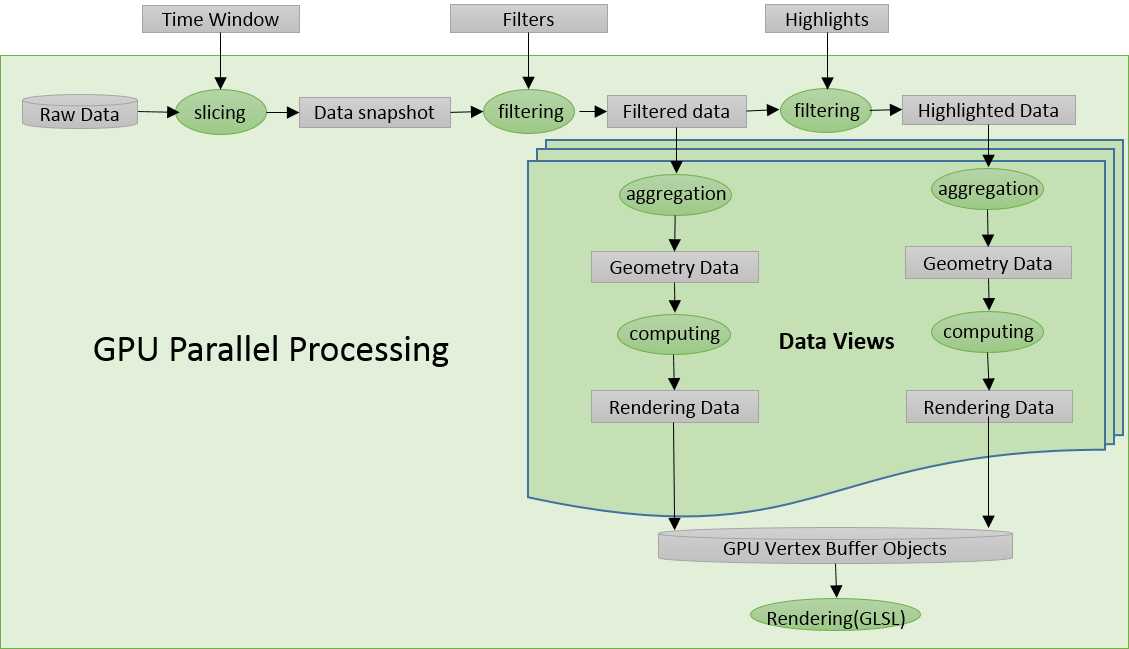
\includegraphics[width=1.0\linewidth]{pic/flow-chart.png}
	\parbox[t]{1.0\columnwidth}{\relax
	}
	%
	\caption{\label{fig:datagraph} The data dependency graph: rectangles represent the data and ovals are the parallel computations. Data filters are generated in the CPU side and transformed to the GPU. All data and computations are done on the GPU. } 
\end{figure} 

\begin{itemize}
	\item \textbf{Data filtering}. Data filters (e.g., \textsl{time window}, \textsl{filters} and \textsl{highlights}) are generated by user interactions in the CPU side, then they are passed to the GPU side.  The GPU pipeline of data filtering is as follows. Firstly,  time window is applied to slice the raw data into data snapshots. Secondly,  filters are applied to data snapshots by removing uninteresting data records. Lastly, highlights  aim to emphasize important data items from the filtered datasets.  
	\item \textbf{Data processing}. The aim of this step is to transform the filtered data records into visual primitives. However, data transformation methods varies considering different data views. We summarize them and character data processing into two stages for each data view: 1) aggregation for generating geometry data (e.g., binning data for histogram view); 2) computation for transforming geometry data into visual primitives  (e.g., the bar height for histogram view).
	\item \textbf{Data rendering}. All generated visual primitives are stored in GPU vertex buffer objects. GLSL (OpenGL shading language) codes generate the ultimate visual results when rendering the visual primitives on the screen (e.g.,  splitting one vertex into four for rendering rectangles by geometry shader,  filling colors in triangles by fragment shader). 
\end{itemize}	
 

 


The data dependency graph has several advantages. Firstly, it follows the cross-filtering design pattern~\cite{weaver2010cross}, where the cross-filtering and coordinated multiple view are coupled together.
Secondly, all data processing and visual rendering can easily be vectorized, and data computations are on the fly. Thirdly,  incremental computing can be applied to exploit temporal and spatial locality. When users play animation, frame-to-frame coherence can be exploited. In such cases, only incremental data need to be considered. Moreover, user interactions are  incremental and interactive. So previous querying results can be reused by next queries. Lastly, the data dependency graph is flexible and extensible. More data filters and data views can easily be extended.
%In all, we formalize the computation flow as a direct acyclic graph (DAG) on the GPU, which is the core part of the GPU-centric design.


~~~~~~~~~~~~~~~~  


